\documentclass{edm_template}
\usepackage{amsmath}
%\usepackage[inline]{trackchanges}
\usepackage{natbib}
\usepackage{multirow}
\usepackage[table,usenames]{xcolor}
\definecolor{hcolor}{rgb}{0.5,0,0.25}
%\usepackage[pdftex,pdfborder={0 0 0},colorlinks=true,allcolors=darkblue]{hyperref}
\usepackage[pdftex,pdfborder={0 0 0},colorlinks=true,allcolors=hcolor]{hyperref}
\usepackage{booktabs}
\usepackage{paralist}
\usepackage[utf8]{inputenc}
\usepackage{soulutf8}
\usepackage{graphicx}
\usepackage{rotating}
\usepackage{soul}
\usepackage{flushend}


\DeclareMathOperator*{\argmax}{argmax} % thin space, limits underneath in displays

\newcommand{\dalite}{\textit{[anonymized for review]}}

\begin{document}
% Copyright
%\setcopyright{acmcopyright}
%\setcopyright{acmlicensed}
%\setcopyright{rightsretained}
%\setcopyright{usgov}
%\setcopyright{usgovmixed}
%\setcopyright{cagov}
%\setcopyright{cagovmixed}


% ISBN
\isbn{}

%\conferenceinfo{EDM 2019}{Montreal, Canada}

\newcommand{\Mem}[1]{\hl{[#1]}}
\newcommand{\Mmathsym}[1]{\mathrm{#1}}

\title{Filtering non-relevant short answers in peer learning applications}

\numberofauthors{4}

\newcommand{\ignore}[1]{}
\ignore{
% 1st. author
\alignauthor
Vincent Gagnon\\
    \affaddr{Polytechnique Montr\'{e}al}\\~\\
% 2nd. author
\alignauthor
Audrey Labrie\\
    \affaddr{Polytechnique Montr\'{e}al}\\
\and
\alignauthor
Sameer Bhatnagar\\
    \affaddr{Polytechnique Montr\'{e}al}\\
\alignauthor
Michel C. Desmarais\\
    \affaddr{Polytechnique Montr\'{e}al}\\
}
\author{
% 1st. author
\alignauthor
1st. author\\
    \affaddr{Institution}\\~\\
% 2nd. author
\alignauthor
2nd. author\\
    \affaddr{Institution}\\
\and
\alignauthor
3rd. author\\
    \affaddr{Institution}\\
\alignauthor
4th. author\\
    \affaddr{Institution}\\
}

\maketitle


\begin{abstract}
Applications that adopt peer instruction and active learning make use of short student answers as a learning opportunity: they take some answers as topics of discussion in class, or select answer rationales from peers to foster self-reflection on the learner's own rationale to a question.  However, experience with these applications reveals that some answers are irrelevant, inappropriate, or could even be offensive, and must therefore be filtered out.  Automatic identification of these rationales is the topic of this research.  We introduce an easy-to-implement approach based on standard text classification techniques, namely bag of words and vector space models, and show its effectiveness for filtering irrelevant answers.
\end{abstract}

\keywords{MOOC, video watching traces, attendance rate, utilization rate, watch index.}

%%%%%%%%%%%%%%%%%%
\section{Introduction}

Recent student response systems (SRS)~\cite{kaleta2007student,farris2017using} allow students to provide free-text answers to short open-ended questions.  These answers can then serve for in-class discussion and feedback, such as in Socrative~\cite{nawalaniec2015socrative}.  They also serve in out-of-class peer-instruction, as in \dalite~\cite{bhatnagar2016dalite} where other student's answer rational are presented to students to nurture self-reflexion on a student's own rational.

Experience with such systems shows that a small proportion of the answers given by students are inappropriate and should not be presented to their peers.  With over 100k answer rationals currently in \dalite, filtering out these answers by reading through them is a daunting task.  With answers that are shown in-class, as with Socrative, pre-screening would take up too much teacher attention and would not scale well to large classes.  An automatic means to filter unwanted answers is therefore paramount to such SRS.

This problem is similar to spam-filtering to the extent that it is a binary classification to filter undesired answers, but it also draws from the problem of automatic short answer grading~\cite{galhardi2018machine} to the extent that desired answers are relate to a topic and to a specific question.  We propose an approach to filter unwanted student answers that uses well known and simple-to-implement techniques and tailors them to this specific aim.

%%%%%%%%%%%%%%%%%%%%%%%%%%%%%%%%%%%%%%%%%%%%%%%%%%%%%%%%%%%%%%%%%%%%%%%%%%%%%
\section{Related work}

Open-ended questions enable teachers to capture student's higher level of understanding than close-ended questions~\cite{reilly2014scoring}. Analysis of short answers in SRS can therefore increase the quality and effectiveness of feedback given by teachers during in-class exercises. 

Previous work on automatic short answer grading has been done using supervised and unsupervised learning techniques. The k-means was proven effective when used on student responses when separating strong from weak answers. On the other end, a successful model built from graded answers is able to predict the grade of a new answer and do no worse than grades assigned  by teachers~\cite{suzen2018automatic}. In the context of the current research, supervised learning is. It would require a set of answers to be graded by teachers which limits the number of possible questions.

Other methods using Latent Semantic Analysis (LSA) and Singular Value Decomposition (SVD) such as the Intelligent Essay Assessor (IEA) \cite{hearst2000debate,Jerrams-Smith+Soh+Callear+2001} were used in essay grading. The IEA was able to provide instantaneous feedback on the student work~\cite{galhardi2018machine}.
%%%%%%%%%%%%%%%%%%%%%%%%%%%%%%%%%%%%%%%%%%%%%%%%%%%%%%%%%%%%%%%%%%%%%%%%%%%%%
\section{Proposed filtering method: bag of words and vector space}

The method rests on the principle that irrelevant student answers will contain words that are unrelated to the ones of the relevant answers.  In that respect, an irrelevant answer is expected to be close to orthogonal to all other answers in a vector space model~\cite{turney2010frequency}.

To measure the general orthogonality of an answer, we average the cosine of each answer with all other answers.  Given a document-term matrix of~$n$ student answers (documents) by~$t$ terms, $\mathbf{A}_{n \times t}$, the average cosine of answers~$d_i$ in corpus~$D$ is defined as:
\[ \overline{\textrm{cos}}_D(d_i) = \frac{\sum_{j \in D} \textrm{cos}(d_i, d_j)}{|D|} \]
where $|D|$ is the corpus size and~$\textrm{cos}(d_i, d_j)$ is the value of the cosine between answers~$d_i$ and~$d_j$.

To create the document-term matrix, $\mathbf{A}_{n \times t}$, we apply the common practice of word stemming and spell correction.  The \texttt{hunspell}\footnote{\url{https://cran.r-project.org/web/packages/hunspell/vignettes/intro.html}} package based on Nemeth's work is used for this purpose~\cite{nemeth2011hunspello}. The term-document matrix is also transformed using the standard TF-IDF calculated from the corpus.  


%%%%%%%%%%%%%%%%%%%%%%%%%%%%%%%%%%%%%%%%%%%%%%%%%%%%%%%%%%%%%%%%%%%%%%%%%%%%%
\subsection{Answer labeling}

The next step is to use the average cosine, $\overline{\textrm{cos}}_D(d_i)$, to determine if an answer is relevant or not.

We can see from Figure~\ref{tab:hist1} that the distribution of the average cosine for relevant and non-relevant answers is bimodal. Figure~\ref{tab:hist1}'s distribution corresponds to a single corpus, but both corpuses show the same bimodal pattern.  This observation leads to a simple approach to determine the non-relevant answers based on clustering.  

Given that non-relevant answers are a small portion of all answers and their average cosine is always lower than the large majority, they tend to cluster around and above~0.  We use the k-means clustering algorithm and take values between~2 and 10~clusters.  The cluster with the closest value to~0 is considered as the non-relevant set of answers.


%%%%%%%%%%%%%%%%%%%%%%%%%%%%%%%%%%%%%%%%%%%%%%%%%%%%%%%%%%%%%%%%%%%%%%%%%%%%%
\subsection{Dimension reduction (M2)}

A common approach to improve semantic similarity search between documents (or words) is to perform dimensionality reduction of the term-document matrix.  LSA is probably the most widely used dimension reduction approach~\cite{dumais2004latent}.  In this variant of M1, the term-document matrix is reduced with SVD using \Mem{ici il faut déterminer le nombre de dimensions---il existe quelques méthodes pour déterminer ce nombre mais on peut le fixer à 50 pour le moment.}


%%%%%%%%%%%%%%%%%%%%%%%%%%%%%%%%%%%%%%%%%%%%%%%%%%%%%%%%%%%%%%%%%%%%%%%%%%%%%
\section{Data sets}

Two corpuses are used in this study.  They cover two context of use and, to a certain extent, two extremes cases: a very small data set with multiple valid open text answers, and a relatively large data set of rationals to a specific answer choice in a multiple choice question.

The first corpus is small and representative of the context where answers must be filtered in real-time as they come in.  The second corpus is from a peer learning environment where filtering can be conducted off-line.  The objective of this environment is to avoid presenting self-reflective rationales that are non-relevant.  The first corpus is typical of \textit{Socrative} whereas the second one is from \textit{\dalite}.  Another factor that differentiates the two corpuses is students were anonymopus in the first context whereas they were not in \textit{\dalite}.

The first corpus is a small set of answers to a single question: ``What are the usabilty issues with the CD-player device''.  The device is shown in Figure~\ref{tab:sanyo} and has a fair number of problems over many dimensions, from \textit{guidance}~\cite{scapin1997ergonomic} to requirements engineering.  The question was proposed to a class of approximately 150~students and the students answered through the \textit{Socrative} application.  Since there are multiple good answers, the answers often reported multiple issues with the devices.  Answers were segmented into single-issue texts by two teacher assistantes.  Inter-judge agreement \Mem{à compléter}.

\begin{figure}
  \centerline{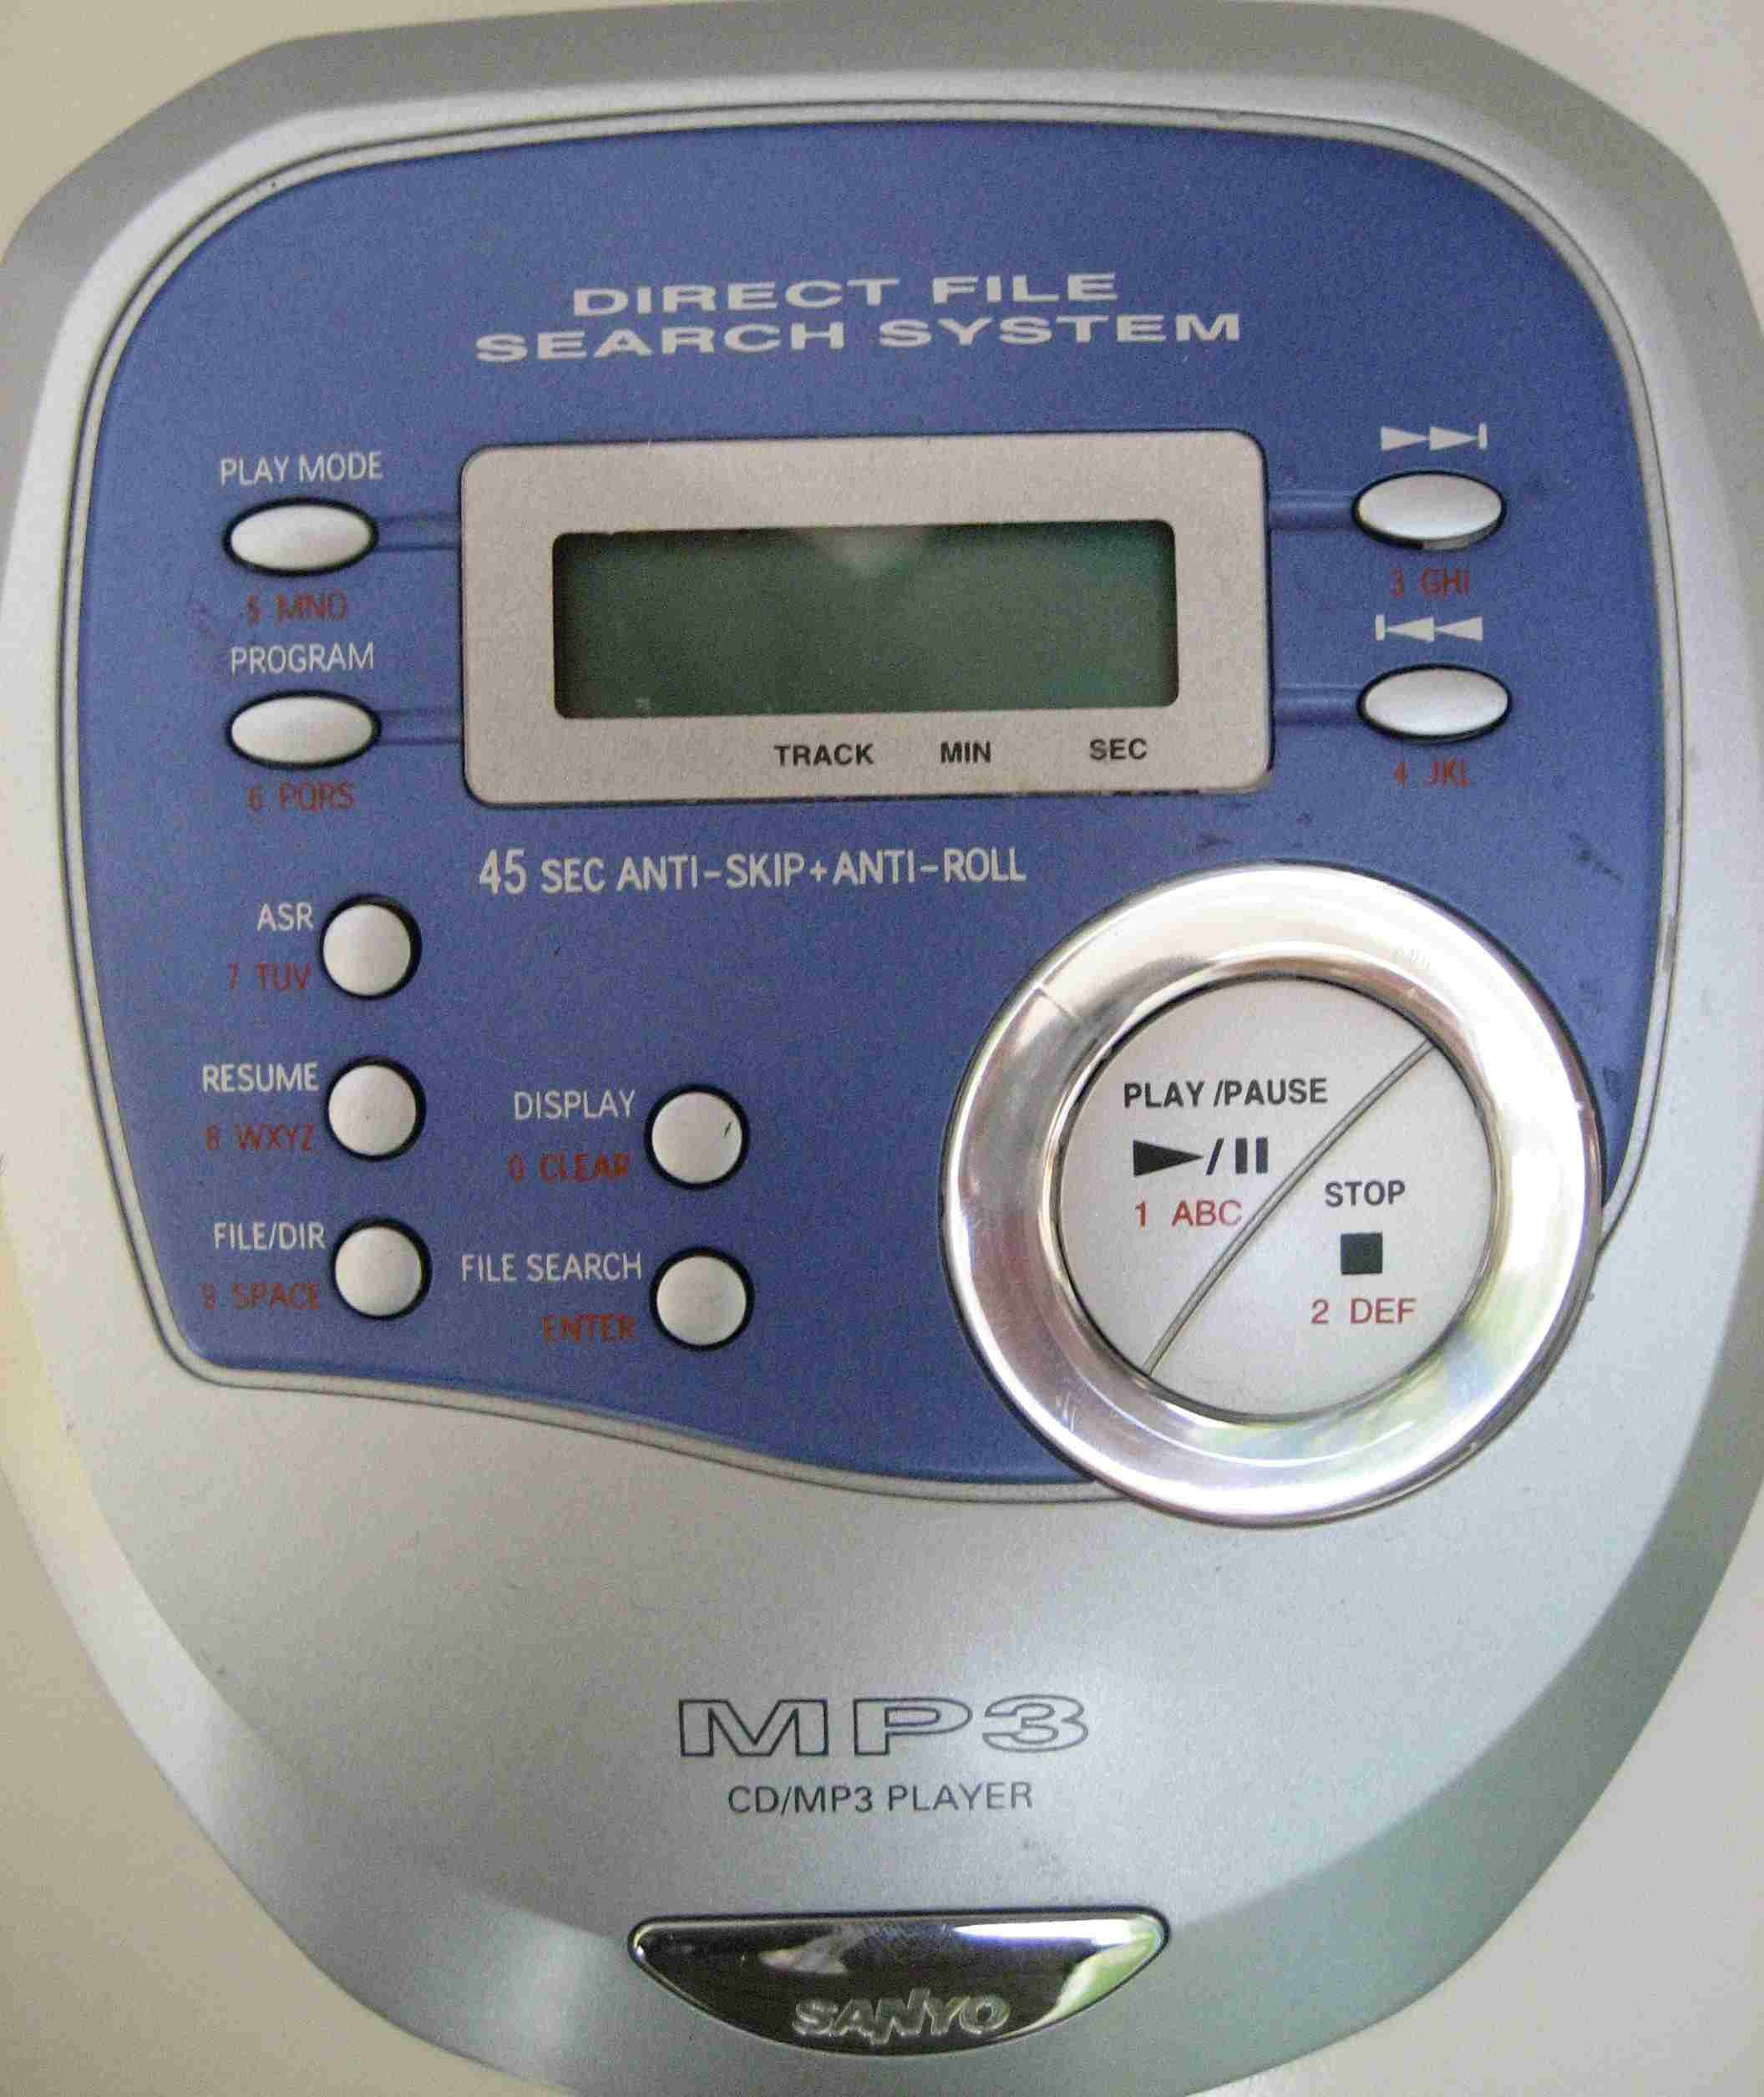
\includegraphics[width=.75\columnwidth]{Images/sanyo-photo.jpg}}
  \caption{Corpus 1: usability issues with an MP3-CD player device.}
  \label{tab:sanyo}
\end{figure}

The second corpus contains a much larger number of student answers and cover six questions.  Segmentation of answers into issues addressed is not relevant in this context.  The answers are taken from a college level physics class.

General statistics on the two corpuses are reported in Table~\ref{tab:corpus}.

\begin{table}
  \caption{Corpus statistics}
  \label{tab:corpus}
  \begin{center}
    \begin{tabular}{rr@{}lr@{}l}
      \toprule
      & \multicolumn{2}{c}{Corpus 1} & \multicolumn{2}{c}{Corpus 2}\\
      \midrule
      Questions & 6&$\,$(1) & 6 \\
      Answers & 229&$\,$(71) & 2054 \\
      Students & 90& & 367 \\
      Non-relevant answers ratio & \multicolumn{1}{r@{}}{12}&\multicolumn{1}{@{}l}{.7$\,$\%} & 13&\multicolumn{1}{@{}l}{.8$\,$\%} \\
      \bottomrule
    \end{tabular}    
  \end{center}
\end{table}

%%%%%%%%%%%%%%%%%%%%%%%%%%%%%%%%%%%%%%%%%%%%%%%%%%%%%%%%%%%%%%%%%%%%%%%%%%%%%
\section{Results}

Figure~\ref{tab:hist1} shows the distribution of average cosines for relevant and non-relevant answers.  The non-relevant answers do have an average cosine that is generally close or equal to~0.  

\begin{figure}
%  \includegraphics[width=\columnwidth]{Images/dalite_mean_distance_10clusters.png}
  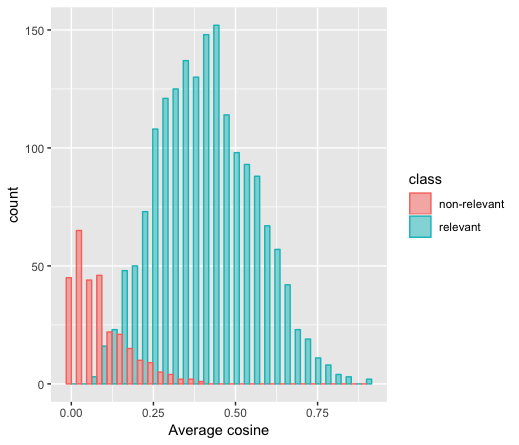
\includegraphics[width=\columnwidth]{Images/dalite_av_cosine_10clusters.png}
  \caption{Histogram of average cosines for relevant and non-relevant student answers.}
  \label{tab:hist1}
\end{figure}

The $F_1$ classification results of the experiments are reported in Table~\ref{tab:res}.  $F_1$ scores are calculated considering non-relevant answers as Positives, since the filtering aims to recall non-relevant as opposed to relevant answers (note that using relevant answers as Positives would give different scores).

The results are broken down by the methods described and compared with a simple baseline that is actually used in \dalite which consists in classifying answers that contain 3~words or less as irrelevant.

\begin{table}
  \caption{Answer filtering results}
  \label{tab:res}
  \begin{center}
    
    \begin{tabular}{lcc}
      \hline
      & \multicolumn{2}{c}{$F_1$ scores}\\
      \cline{2-3}
            {Method} & Corpus 1 & Corpus 2\\
            \hline
            M1 & 0.839 & x \\
            M2 & x & x \\
            M3 & x & x \\
            3-words rule & 0.797 & 0.250 \\
            \hline
    \end{tabular}
  \end{center}
\end{table}
%% rule3 <- (sapply(strsplit(as.character(mydalite_data$Explication), " "), length))<4
%% F1_Score(!rule3,!(rater2=='x' | rater2=='xx'))



%%%%%%%%%%%%%%%%%%%%%%%%%%%%%%%%%%%%%%%%%%%%%%%%%%%%%%%%%%%%%%%%%%%%%%%%%%%%%
\section{Conclusion}





\bibliographystyle{plain}
\bibliography{ref.bib}
\end{document}
